\subsubsection{Total number of messages sent}\label{subsubsec:ld2krmessages}

This is an indication of the energy efficiency of the entire network.

The maximum number of copies is the dominant factor (\(85.18\%\)), as in the
high density case. In the previous case the size of the hear window was the
second most important factor. Here, instead, we have the broadcast radius
(\(6.57\%\)) and its combination with the maximum number of copies. The
unexplained variation is extremely low \(0.31\%\).

From \figref{fig:ldperfmessagesR} we notice that increasing the broadcast radius
is useful to reduce the total number of messages sent when the maximum number of
copies is low. This can be explained by the fact that with an higher value for
\(m\) means that nearly all the users in the network will relay the message
after they have successfully heard it. So, if \(m\) is high, there is not much
to do to reduce the total number of messages sent.

\begin{figure}[htb]
	\centering
	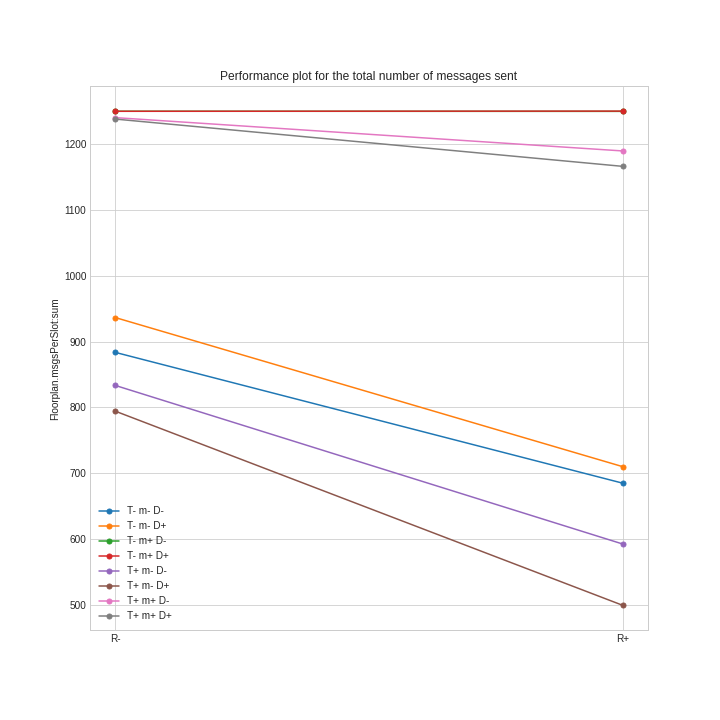
\includegraphics[width=0.6\textwidth]{img/ld/messages-R-perfplot}
	\caption{Performance plot for the total number of messages sent. The
	broadcast radius can be used to reduce the total number of messages sent
	when the maximum number of copies is not
	high}\label{fig:ldperfmessagesR}
\end{figure}
